\documentclass{chi2009}
\usepackage{times}
\usepackage{url}
\usepackage{graphics}
\usepackage{color}
\usepackage[pdftex]{hyperref}
\hypersetup{%
pdftitle={TwinList: \\ Visualizing List Differences},
pdfauthor={Leonardo Max Baptista Claudino, claudino@cs.umd.edu \\
	    Sameh Khamis, sameh@cs.umd.edu \\
	    Ran Liu, ranliu@cs.umd.edu \\
	    Ben London, blondon@cs.umd.edu \\
	    Jay Pujara, jay@cs.umd.edu},
pdfkeywords={list visualization},
bookmarksnumbered,
pdfstartview={FitH},
colorlinks,
citecolor=black,
filecolor=black,
linkcolor=black,
urlcolor=black,
breaklinks=true,
}
\newcommand{\comment}[1]{}
\definecolor{Orange}{rgb}{1,0.5,0}
\newcommand{\todo}[1]{\textsf{\textbf{\textcolor{Orange}{[[#1]]}}}}

% TwinList Macros
\newcommand{\TwinList}{\textsc{TwinList}}
\newcommand{\ListViewer}{\textit{List Viewer}}
\newcommand{\AcceptReject}{\textit{Accept/Reject}}
\newcommand{\AcceptedRejected}{\textit{Accepted/Rejected}}
\newcommand{\Controls}{\textit{Control Panel}}
\newcommand{\Filters}{\textit{Filter Panel}}
\newcommand{\Details}{\textit{Details Panel}}
\newcommand{\GroupBy}{\textit{Group By}}
\newcommand{\SortBy}{\textit{Sort By}}

\pagenumbering{arabic}  % Arabic page numbers for submission.  Remove this line to eliminate page numbers for the camera ready copy

\begin{document}
% to make various LaTeX processors do the right thing with page size
\special{papersize=8.5in,11in}
\setlength{\paperheight}{11in}
\setlength{\paperwidth}{8.5in}
\setlength{\pdfpageheight}{\paperheight}
\setlength{\pdfpagewidth}{\paperwidth}

% use this command to override the default ACM copyright statement 
% (e.g. for preprints). Remove for camera ready copy.
\toappear{Submitted for CMSC 734 Information Visualization.}

\title{TwinList: \\ Visualizing List Differences}
\numberofauthors{5}
\author{
  \alignauthor Leonardo Max Batista Claudino \\
    \affaddr{Dept. of Computer Science, University of Maryland}\\
    \affaddr{College Park, MD 20742}\\
    \email{claudino@cs.umd.edu}
  \and
  \alignauthor Sameh Khamis\\
    \affaddr{Dept. of Computer Science, University of Maryland}\\
    \affaddr{College Park, MD 20742}\\
    \email{sameh@cs.umd.edu}
  \and
  \alignauthor Ran Liu \\
    \affaddr{Dept. of Computer Science, University of Maryland}\\
    \affaddr{College Park, MD 20742}\\
    \email{ranliu@cs.umd.edu}
  \and
  \alignauthor Ben London \\
    \affaddr{Dept. of Computer Science, University of Maryland}\\
    \affaddr{College Park, MD 20742}\\
    \email{blondon@cs.umd.edu}
  \and
  \alignauthor Jay Pujara \\
    \affaddr{Dept. of Computer Science, University of Maryland}\\
    \affaddr{College Park, MD 20742}\\
    \email{jay@cs.umd.edu}
}

\maketitle

\begin{abstract}
We present a novel list visualization tool named $\TwinList$, for the purpose of list visualization and matching. Leveraging Adobe's Flex platform and the Prefuse Flare toolbox, we created a rich internet application (RIA) with dynamic animated effects. These animated transitions lead the user through the procedure of matching two lists, using color coding to highlight the similarities and differences between the two. List items can be grouped, sorted and filtered according to their attribute values, to enhance workflow. To illustrate the efficacy of the application, we conduct usability testing with several doctors and peers.
\end{abstract}

\keywords{list visualization} 

\category{H.5.2}{Information Interfaces and Presentation}{Miscellaneous}

\section{Introduction}
In applications involving list-based data, it is often necessary to match similar items and take some action on the list elements. One such domain is that of medical list reconciliation, in which a physician must reconcile a patient's medication from multiple prescribers. Another application might be comparing bag-of-words data from multiple text corpora.

\subsection{Related Work}

\section{TwinList}
$\TwinList$ is a novel list visualization tool for the purpose of illustrating the similarities and differences between two lists. It can be used in many cases where the comparison of two lists of items is required. The primary application that $\TwinList$ supports is that of medication list reconciliation: comparing and reconciling multiple medications that have been prescribed to a patient from multiple sources\cite{JCAHO-2006}. However, $\TwinList$ is equally adept in other applications, such as comparing bag-of-words lists or visualizing \todo{Jay, what is that bio data you have?}. 

$\TwinList$ interface consists of four major components: the $\ListViewer$, $\Controls$, $\AcceptedRejected$ lists and $\Details$, as shown in (Figure~\ref{fig:interface}).

%\begin{figure}
%\begin{center}
%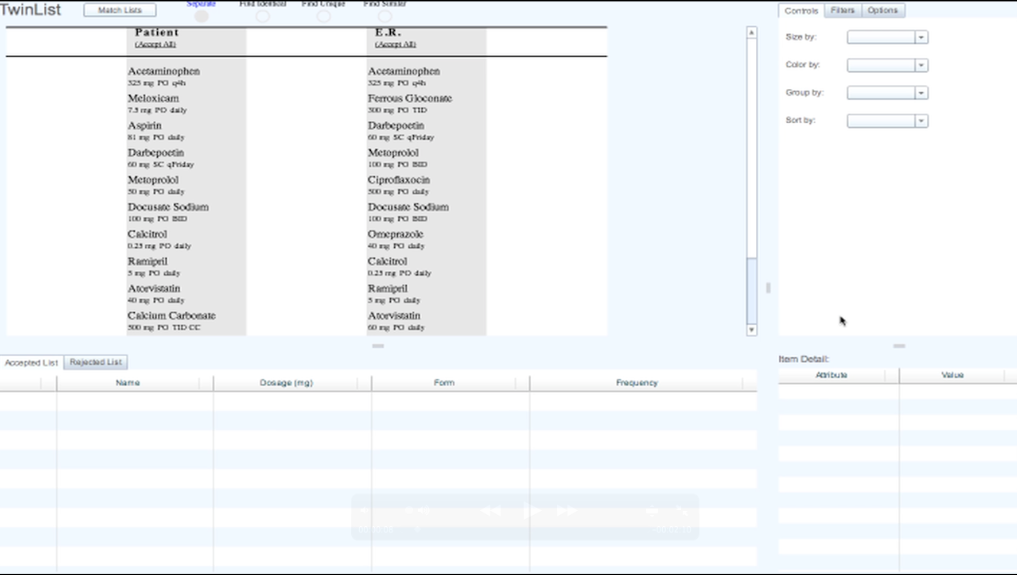
\includegraphics[width=1.1\linewidth]{interface}
%\end{center}
%   \caption{$\TwinList$ interface}
%   \label{fig:interface}
%\end{figure}

\subsection{ListViewer}

\subsection{Controls}

\subsection{Filters}

\subsection{Options}

\section{Evaluation}
Our goal was to deliver a working prototype, not a finished, fully-functional application. As such, we are more concerned with qualitative than quantitative feedback on the features of our visualization system at this point. According to the categorization proposed by Lam et al~\cite{lam-bertini-isenberg-plaisant-carpendale-2011}, the evaluation scenario best matching our present purposes is the \textit{User Experience (UE)} test case. The goal of the following experiments is to observe how users react to the visualization and interaction features offered by $\TwinList$. We will use their feedback to improve the system's design in future versions.

\subsection{Experiment Design}
Our test subjects came from two populations: two physicians and two non-specialist participants. The former used $\TwinList$ to perform medication reconciliation; the latter to fine interesting insights in bag-of-words data from two State of Union speeches. The testing protocol proceeded as follows: first, the user watched a $~7$-minute video demonstrating basic usage. Following this, the user was allowed to ask questions. Next, the user interacted with the system unaided, performing either specific tasks (medication reconciliation case studies) or exploratory analysis (State of the Union comparison). While using the system, subjects were encouraged to \textit{think aloud}.\todo{maybe a ``think aloud" citation here?} The entire experiment was captured in both audio and screen capture video.

\subsection{Case 1: Med. reconciliation, A. Z. H., male, 34 y. o.}
Overall, the participant performed the tasks as expected and reported anticipated results. A. Z. H. purported to be very comfortable with computers. He does not perform medication reconciliation on a regular basis, except when doing inpatient aid and discharge from the hospital, for which he does not use any software. This is how he describes his $\TwinList$ experience: \textit{``It's really impressive, the way you organize things is great. It's definitely a step in the right direction \dots"}. He was very enthusiastic and provided several suggestions, most of all worth including in this section. 

\subsubsection{Results}
This is our reading of A. Z. H.'s experience:
\begin{itemize}
\item There is need for an indication that there are more items than what can be currently seen in a column. The scroll bar alone is insufficient.
\item It is difficult to get to the $\AcceptReject$ pop-up menu when accepting/rejecting an item. He had trouble with the click-and-hold behavior, wanting instead to use the mouse's right-click button.
\item To send items from $\AcceptedRejected$ lists back to the viewer one-by-one requires quite some effort when you have many items in those lists. A \textit{Remove All} button would be desirable.
\item Warning dialogs or undo may be needed when accepting and rejecting items, since it is a delicate operation in medication reconciliation.
\item In the control panel, drop-down boxes should indicate what the default $\GroupBy$/$\SortBy$ attributes are, instead of blank captions. (The default is actually the original ordering.)
\item It would be desirable to shorten vertical empty spaces in between items to minimize the need of scrolling.
\item The number of visible item attributes should be shortened in the $\ListViewer$, since reconciliation is performed, in practice, based on only a few (e. g. the \textit{Indication} feature).
\item For items in the \textit{Similar} columns, the item pop-up menu should have a third option, to automatically reject an item of a list if its counterpart at the other list was accepted. According to the participant, this would be the likely outcome in almost every such context.
\item The participant suggested that we should change the way items are displayed so that, for each list, you have items sorted by some \textit{uniqueness level}; for example, by vertically ranging from identical to unique. This would add more meaning to the vertical structure of the list, which is somewhat lost after lists are matched, but would represent a significant change in the concept.
\item The participant felt that placing the $\AcceptedRejected$ lists at the bottom of the interface may be suboptimal for tracking what happened to processed items, especially when the user gets distracted.
\item The participant missed being able to interact on the spot with accepted/rejected items that are grayed out. In his words: \textit{``If it is grayed out, what if (\dots) I really want to do the 100 mg, is there any way to click and have it re-instate (\dots) or un-reject/un-accept"}. He believes that if he could interact with grayed-out items on the viewer, the $\AcceptedRejected$ lists might not even be necessary, thus allowing more room for the main visualization. As such, the list of rejected/accepted items could be output as the final product of the interactive process and would be activated by pressing a button. As he suggested: \textit{``\dots Here is your final list of medications, this is your rejected list over here, and when one finally accepts, export to (\dots) or put in patient's medical record \dots"}.
\item The participant suggested an additional \SortBy criteria: in his own words, \textit{``medications that haven't been dealt with yet."} We translate this as a grouping of medications based on their accepted/rejected status. This is a useful, general concept applicable to other list matching problems.
\item The participant mentioned the importance of filters, especially to filter by route (e.g. I.V. medications).  
\end{itemize}

\section{Conclusion}

\bibliographystyle{abbrv}
\bibliography{twinlist}

\end{document}
